\section{Experimental results} \label{experiments}

\subsection{Dataset insights}  \label{ch:experimentsA}

This chapter presents the dataset insights of the complete dataset with full genome sequences and the dataset insights of the preprocessed dataset.

\subsubsection{Complete dataset}  \label{ch:experimentsAa}

The dataset consists of 9199 parent child pairs.
The distribution how the parent and child sequences differ can be seen in figure \ref{distributionDifferencesParentChild}. The majority of parent child pairs differ in less than 200 characters. The number of completely equal parent child pairs is 396.

\begin{figure}[ht]
	\centering
	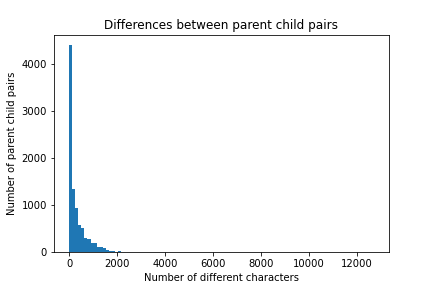
\includegraphics[width=0.7\linewidth]{figures/distributionDifferencesParentChild.png}
	\caption{Distribution of the differences between parent and child sequences \cite{own representation}}
	\label{distributionDifferencesParentChild}
\end{figure}

Figure \ref{mutatedGeneticLoci} visualizes the distribution of mutations over the full \ac{SARS-CoV-2} genome.

\begin{figure}[ht]
	\centering
	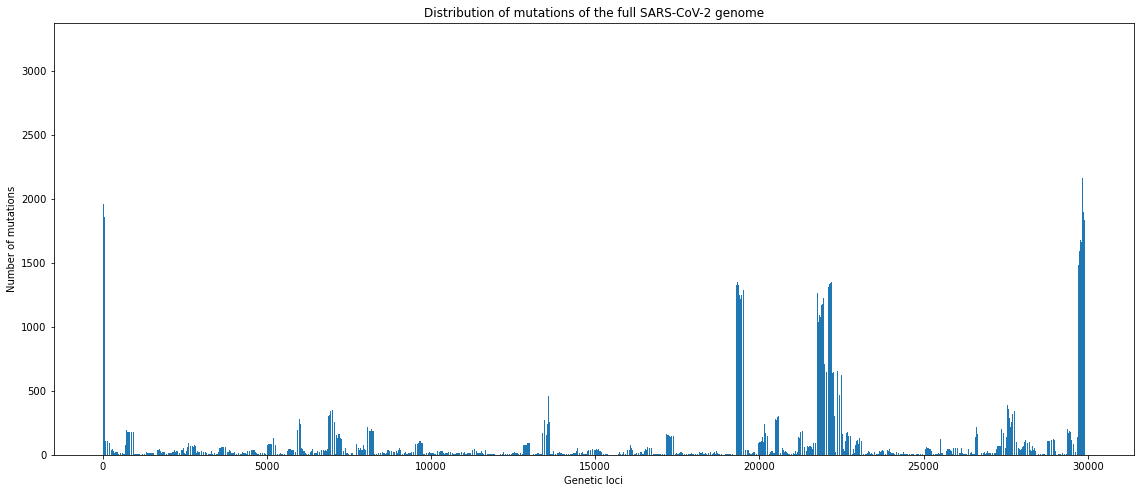
\includegraphics[width=1.0\linewidth]{figures/mutatedGeneticLoci.png}
	\caption{Mutated genetic loci \cite{own representation}}
	\label{mutatedGeneticLoci}
\end{figure}

Based on this distribution -> subpart selection in preprocessing


\subsubsection{Preprocessed dataset}  \label{ch:experimentsAb}

The complete dataset is preprocessed as described in chapter \ref{ch:approachB}.
The distribution how the parent and child amino acids differ in the selected subpart can be seen in figure \ref{preprocessedDistributionDifferencesParentChild}. The majority (6946) of parent child pairs are equal.

\begin{figure}[ht]
	\centering
	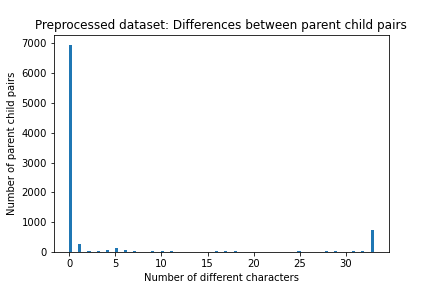
\includegraphics[width=0.7\linewidth]{figures/preprocessedDistributionDifferencesParentChild.png}
	\caption{Preprocessed dataset: Distribution of the differences between parent and child sequences \cite{own representation}}
	\label{preprocessedDistributionDifferencesParentChild}
\end{figure}

Figure \ref{preprocessedMutatedGeneticLoci} visualizes the differing amino acids and their positions of the selected subpart of the \ac{SARS-CoV-2} genome. They are distributed equally over the selected subpart.

\begin{figure}[ht]
	\centering
	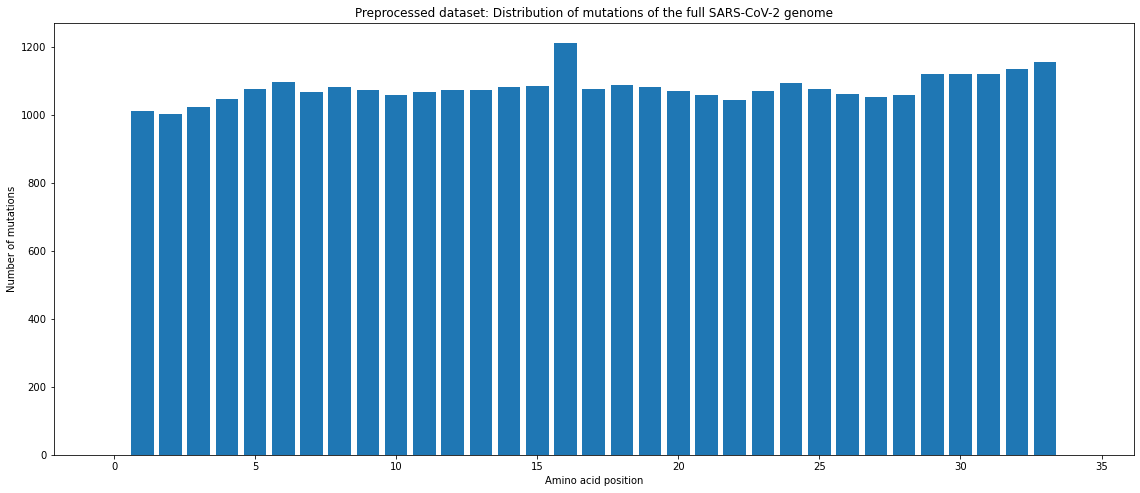
\includegraphics[width=1.0\linewidth]{figures/preprocessedMutatedGeneticLoci.png}
	\caption{Preprocessed dataset: Differing amino acid positions \cite{own representation}}
	\label{preprocessedMutatedGeneticLoci}
\end{figure}

Based on this distribution -> subpart selection in preprocessing


\subsection{Evaluation}  \label{ch:experimentsB}


% Define what is a correct mutation prediction, see MutaGAN paper - Generator Evaluation
% Define Evlauation metrics, see MutaGAN paper - Generator Evaluation
% Evaluation chaper of MutaGAN very well written, will be inspiring
% Compare our performance to those of other papers

\newpage
